\label{sec:breakout}
Here the agent needs to master the atari game breakout, see \autoref{fig:breakout}. The agent controls a small bar at the bottem of the screen with possible actions: move left, move right or stay. A ball moves with constant speed through the envirement. If the agent positions the small bar such that the ball hits the bar the ball inverts its vertical velocity bouncing upwards. Whenever the ball hits the bottem of the screen it disappears, the agent loses a life (it starts with 5) and a new ball is introduced with a random direction downwards. When the ball hits the left and right side of the screen the horizontal velocity is inverted making it bounce of the walls. Somewhat below the top of the screen is a stack of rows of blocks. Whenever the ball hits one of the blocks: the block disappears, the ball inverts its vertical velocity and the agent is rewarded with score one for the current timestep. If the ball hits the top of the screen its vertical velocity is inverted, bouncing it off the top. 

\begin{marginfigure}
    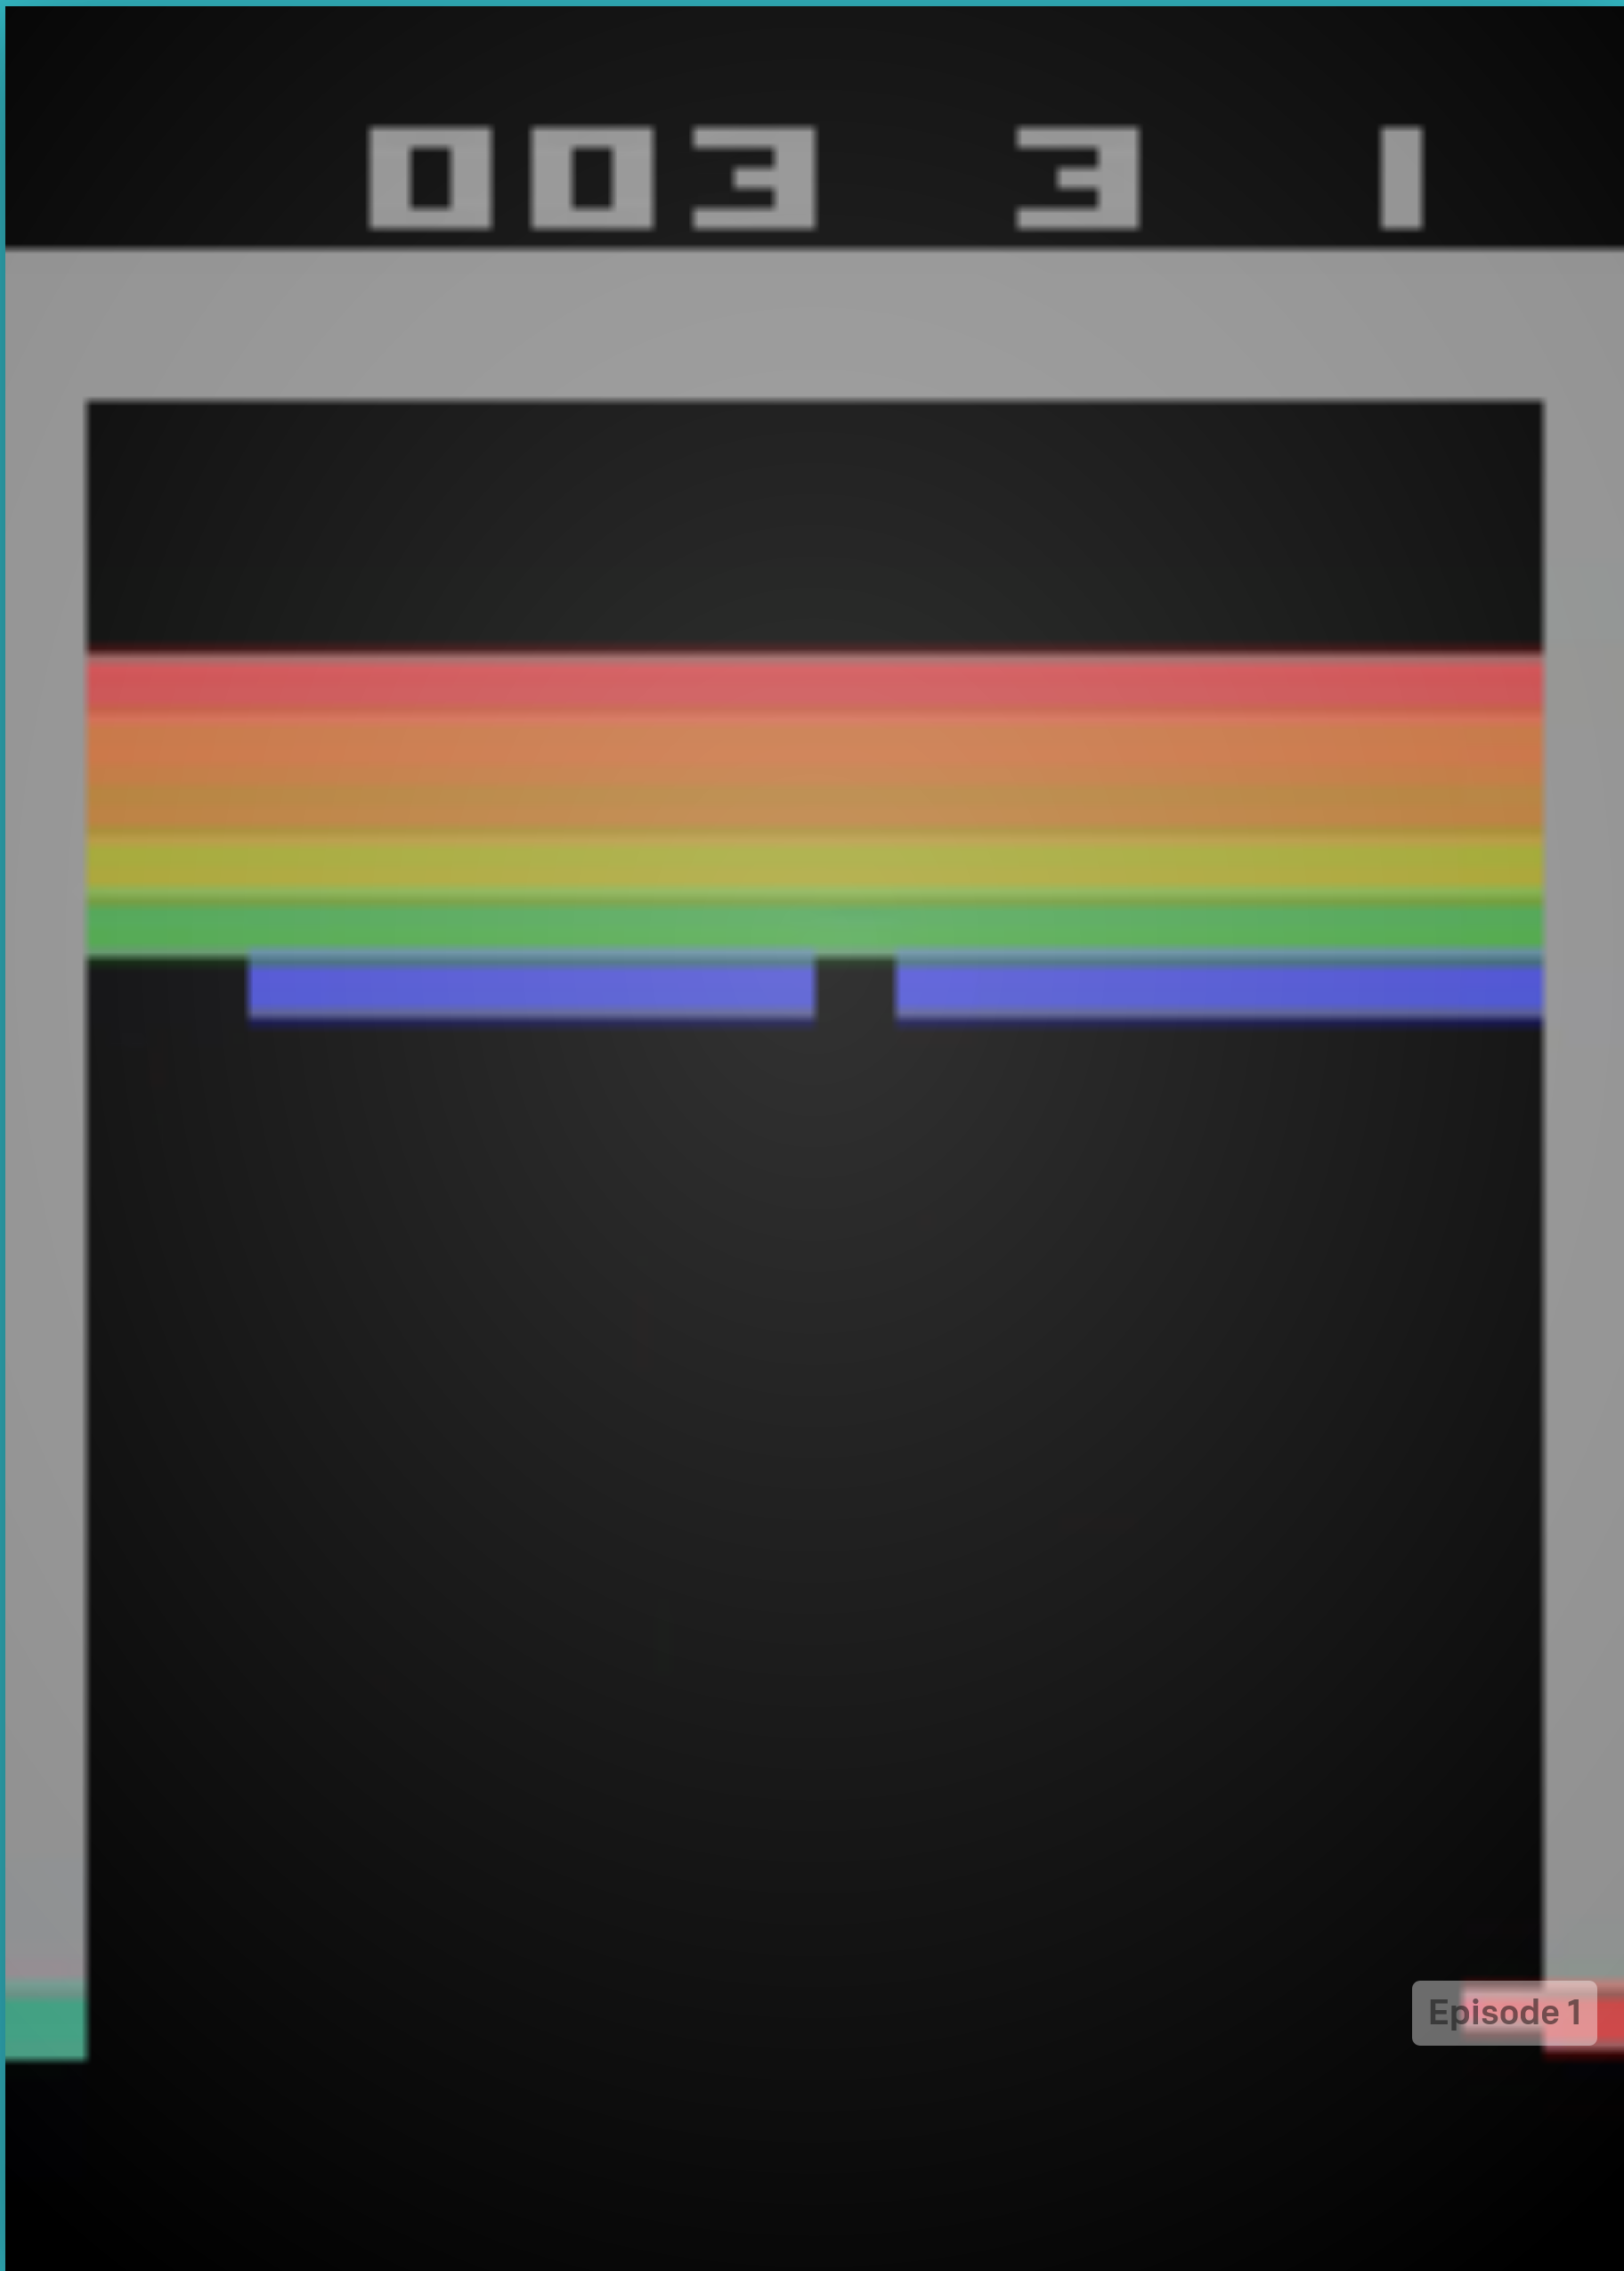
\includegraphics{breakout}
    \caption{The atari breakout envirement}
    \label{fig:breakout}
\end{marginfigure}

In this problem agent gets the same information as a human would, the pixels on the screen. Aditionally we give it the reward of the current timestep. Due to the computational complexity we do not want the agent to process the whole screen each timestep. We build our implementation on top of the \texttt{BreakoutDeterministic-v4} envirement provided by the \textit{openAI gym} project. This envirement returns the game state only once every 4 frames lowering the computational requirements.

\subsection{Implementation}
Initially we used a slightly adapted version of the mountain car DQN implementation described in \autoref{sec:mcar_impl}. The simple multilayer dense neural network was replaced with a convolutional neural network consisting of 2 layers both with kernal size 3 followed by two dense layers. The frames from the envirment where changed to greyscale and cropped to $80$ by $72$ pixels. This leaves the game envirement intact but removes the score at the top and ornamental edges, leaving an images as in \autoref{fig:breakout_postprocess} for the network.

This did not result in any learning by the agent. I tried multiple different networks before taking a look at related literature\cite{atari}. This lead to the conclusion that my agent was that my hyper paramaters where far from where they should be.

Taking the hyperparamaters from the famouse "Human-level control through deep reinforcement learning"\cite{DQN} we start changing the implementation. The mountain car agent is limited in the number of training sessions, this does not make sense for the breakout agent as we want to limit the number of steps not training sessions. From the perspective of a human traning there is no difference between losing a life and the game restarting however the agent was not even punished for losing a life. That was changed so losing a life is treated as losing the game during training.
Using only one frame as input to the network does not allow the agent to use the concept of direction or speed, essential to a human player. As in\cite{DQN} we feed the network a stack of the last 4 frames, as given to us by the envirement, for prediction and during training. 

\begin{marginfigure}
    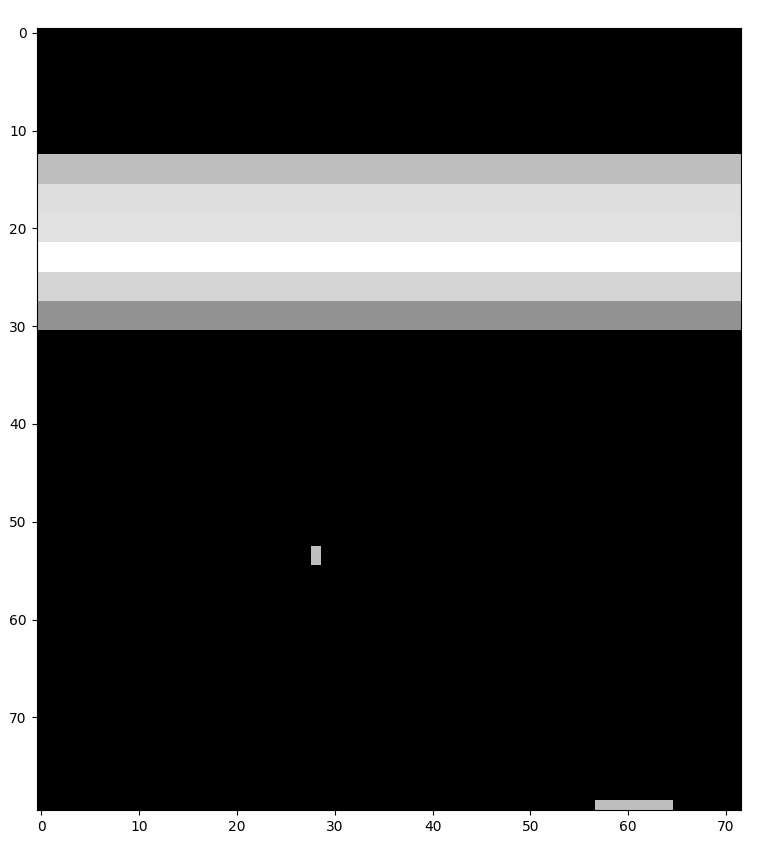
\includegraphics{network_input}
    \caption{A frame returned by the atari breakout envirement after postprocessing for our agent, converting to color and cropping out the unneeded edges}
    \label{fig:breakout_postprocess}
\end{marginfigure}

These changes give a number of implementation problems. We can not take any action for the first 3 timesteps as we can not make a stack of 4 frames to feed the agent. We have removed the training in sessions however we should not use frames from another training session. For example is the games has ended in frame $x$ we can not use the network until frame $x+4$. To enforce this we use the function \texttt{reset}. It resets the envirement and forwards the game 3 timesteps without taking any action. We use a new class \texttt{State} to keep track of the 4 frames. I provides a method \texttt{push} that takes as arguments an before and after state together with the action taken, score and if the game is over. It then forgets the oldest before and after state adding the new state to its internal stack.
%
This introduced a new problem, the stack of images drastically increased the memory requirements of the agent. Instead of single images the \texttt{event} inserted into the memory (see \autoref{sec:mcar_impl}) are a lot larger at $184$kB per state\footnote{frame before and after an action each $4$ images of $72\cdot80$ pixels, each pixel represented as a python floating point number of $8$ bytes giving a total of $184$kB per state. Multiplied by a million that becomes gigabytes}. If we want to have a replay buffer as in the literature\cite{DQN} of 1 million states the agent would need at least 184 gigabytes. I solved this in two steps. Instead of storing the pixels in the default floating point format they are stored as bytes. This does not lead to significant data loss as the envirment uses one byte per color per pixel, since we are using grayscale we can use a single byte per pixel. The \texttt{State} class is modified to cast pixels to bytes when a new frame is pushed. The \texttt{Predictor} class (see \autoref{sec:mcar_impl}) casts the pixels back to floats before feeding them to the convolutional neural network. By lowering the replay buffer size from one million to \nicefrac{1}{4} million. Later after the agent was run for 10 million steps the memory use was further reduced no longer saving 8 frames for each state but only two and recreating the full 8 frame states as they are sampled from the memory.
%
The \texttt{Epsilon} class constuctor was rewritten, now the decay is not a constant but rather determined by the number of steps that epsilon should decay over from its starting value to its final value.
%
Finally we took the network architecture from the deepmind paper\cite{DQN} after our own would not let the agent learn. It consists of 2 convolutional layers, the first has 16 filters with square kernals size 8 using a stride of 4. The second convolutional layer has 32 filters with square kernals of size 4 and uses a stride of 2. There layers are followed by a fully connected layer and then the fully connected output layer, the first with 256 nodes and the second 4, the number of actions for the environment. Except for the output layer all layers use the rectified linear unit as activation function.